\section{هدف تمرین}
در این تمرین، یک ضرب‌کننده‌ی اعداد مختلط پارامتری در \lr{Verilog} طراحی می‌کنیم. این ماژول دو عدد مختلط $A$ و $B$ را دریافت می‌کند و بسته به سیگنال کنترلی \code{conj}، یا حاصل‌ضرب معمولی $A \times B$ یا $A \times B^*$ را محاسبه می‌کند. تمام ورودی‌ها و خروجی‌ها به صورت \lr{signed} در نمایش \lr{two's complement} هستند.

\section{توضیح معماری}
مدار یک \lr{pipeline} دو مرحله‌ای \lr{synchronous} است. در هر لبه‌ی بالارونده‌ی ساعت، ورودی‌های \code{Ar}، \code{Ai}، \code{Br}، \code{Bi} و \code{conj} در رجیسترهای داخلی لچ می‌شوند. چهار \lr{wire} \lr{combinatorial} (\code{ArBr}، \code{AiBi}، \code{ArBi}، \code{AiBr}) حاصل‌ضرب‌های جزئی را از روی همین رجیسترها محاسبه می‌کنند، و در همان لبه‌ی ساعت \code{Yr} و \code{Yi} نیز آپدیت می‌شوند. از آن‌جایی که هر دو انتساب \lr{non-blocking} هستند، محاسبه‌ی خروجی‌ها از مقادیر ذخیره شده‌ی چرخه‌ی قبل انجام می‌گیرد؛ بنابراین خروجی با تأخیر ۲ سیکل نسبت به ورودی ظاهر می‌شود.

\section{توضیح کد}

\subsection{ماژول \code{complex\_multiplier} (\code{DSD\_HW5\_Q1.v})}
کد ماژول (بدون \lr{port declarations}) به این صورت می‌باشد:

\begin{latin}
    \begin{lstlisting}[language=Verilog]
// registers fot latching the inputs
reg signed [IN_WIDTH-1:0] Ar_reg, Ai_reg;
reg signed [IN_WIDTH-1:0] Br_reg, Bi_reg;
reg conj_reg;

// Intermediate products: 15-bit signed * 15-bit signed = 30-bit signed
wire signed [29:0] ArBr = Ar_reg * Br_reg;
wire signed [29:0] AiBi = Ai_reg * Bi_reg;
wire signed [29:0] ArBi = Ar_reg * Bi_reg;
wire signed [29:0] AiBr = Ai_reg * Br_reg;

always @(posedge clk) begin
    // synchronous reset
    if (rst) begin
        Ar_reg   <= {IN_WIDTH{1'b0}};
        Ai_reg   <= {IN_WIDTH{1'b0}};
        Br_reg   <= {IN_WIDTH{1'b0}};
        Bi_reg   <= {IN_WIDTH{1'b0}};
        conj_reg <= 1'b0;
        Yr       <= {OUT_WIDTH{1'b0}};
        Yi       <= {OUT_WIDTH{1'b0}};
    end else begin
        // 1: latch inputs to the registers
        Ar_reg <= Ar; Ai_reg <= Ai;
        Br_reg <= Br; Bi_reg <= Bi;
        conj_reg <= conj;

        // 2: calculate outputs using values in the registers
        if (!conj_reg) begin
            Yr <= ArBr - AiBi;
            Yi <= ArBi + AiBr;
        end else begin
            Yr <= ArBr + AiBi;
            Yi <= AiBr - ArBi;
        end
    end
end
\end{lstlisting}
\end{latin}

پارامترهای \code{IN\_WIDTH} و \code{OUT\_WIDTH} (با مقادیر پیش‌فرض ۱۵ و ۳۱) ابعاد ورودی و خروجی را تنظیم می‌کنند. با فعال شدن \code{rst}، تمام \lr{register}ها صفر می‌شوند. در غیر این صورت، ابتدا ورودی‌ها لچ می‌شوند و سپس، چون \lr{non-blocking assignment} مقادیر \lr{register} را صرفاً در انتهای سیکل اعمال می‌کند، خروجی‌ها از روی مقادیر سیکل قبل محاسبه می‌شوند. تعریف صریح ابعاد \lr{wire}های جزئی به ۳۰ بیت (دقیقاً کافی برای ضرب دو عدد ۱۵ بیتی \lr{signed}) هم از ابهام در \lr{sign extension} جلوگیری می‌کند و هم منطق \lr{combinatorial} را از منطق \lr{sequential} جدا می‌کند.

\subsection{تست‌بنچ (\code{DSD\_HW5\_Q1\_tb.v})}
\lr{task} اصلی تست‌بنچ به این صورت است:

\begin{latin}
    \begin{lstlisting}[language=Verilog]
task run_test;
    input signed [IN_WIDTH-1:0] in_Ar, in_Ai;
    input signed [IN_WIDTH-1:0] in_Br, in_Bi;
    input in_conj;
    integer exp_Yr, exp_Yi;
    begin
        test_num = test_num + 1;
        Ar = in_Ar; Ai = in_Ai; Br = in_Br; Bi = in_Bi; conj = in_conj;
        @(posedge clk); @(posedge clk); #1;

        if (in_conj == 1'b0) begin
            exp_Yr = ($signed(in_Ar)*$signed(in_Br)) - ($signed(in_Ai)*$signed(in_Bi));
            exp_Yi = ($signed(in_Ar)*$signed(in_Bi)) + ($signed(in_Ai)*$signed(in_Br));
        end else begin
            exp_Yr = ($signed(in_Ar)*$signed(in_Br)) + ($signed(in_Ai)*$signed(in_Bi));
            exp_Yi = ($signed(in_Ai)*$signed(in_Br)) - ($signed(in_Ar)*$signed(in_Bi));
        end

        if (Yr == exp_Yr && Yi == exp_Yi) begin
            passed = passed + 1;
            $display("[PASS] Vector %0d: ...", test_num, ...);
        end else begin
            failed = failed + 1;
            $display("[FAIL] Vector %0d: ...", test_num, ...);
        end
    end
endtask
\end{lstlisting}
\end{latin}

این \lr{task} ابتدا ورودی‌ها را \lr{set} می‌کند، دو \lr{posedge} صبر می‌کند (یک سیکل برای لچ شدن ورودی‌ها، یک سیکل برای آپدیت خروجی‌ها) و یک نانوثانیه بعد از آخرین لبه نمونه‌برداری می‌کند تا از \lr{race condition} جلوگیری شود. مقدار مورد انتظار داخل همان \lr{task} با یک \lr{reference model} محاسبه و با خروجی مقایسه می‌شود.

قبل از شروع تست‌ها، یک چک مجزا برای حالت \lr{reset} انجام می‌شود:

\begin{latin}
    \begin{lstlisting}[language=Verilog]
    @(posedge clk);
    rst = 0;
    @(posedge clk); #1;
    test_num = test_num + 1;
    if (Yr === 0 && Yi === 0)
        $display("[PASS] Vector %0d (reset check): Yr=%0d, Yi=%0d",
                 test_num, Yr, Yi);
    else
        $display("[FAIL] Vector %0d (reset check): ...", test_num);
\end{lstlisting}
\end{latin}

بلافاصله بعد از آزاد شدن \code{rst}، بررسی می‌شود که \code{Yr} و \code{Yi} هر دو صفر هستند.

تست‌های اصلی به ترتیب زیر هستند:

\vspace{0.8cm}
\begin{latin}
    \begin{lstlisting}[language=Verilog]
run_test(15'sd10, 15'sd5,  15'sd4,  15'sd3,  1'b0);
run_test(15'sd10, 15'sd5,  15'sd4,  15'sd3,  1'b1);
\end{lstlisting}
\end{latin}

\vspace{-0.2cm}
ضرب عادی و مزدوج برای اعداد با مؤلفه‌های مثبت؛ هر دو مُد \code{conj} با همان ورودی تست می‌شوند.
\vspace{0.8cm}

\begin{latin}
    \begin{lstlisting}[language=Verilog]
run_test(-15'sd8, -15'sd6, -15'sd3,  15'sd2,  1'b0);
run_test(-15'sd8, -15'sd6, -15'sd3,  15'sd2,  1'b1);
\end{lstlisting}
\end{latin}

\vspace{-0.2cm}
همین تست‌ها برای مؤلفه‌های منفی.
\vspace{0.8cm}

\begin{latin}
    \begin{lstlisting}[language=Verilog]
run_test(15'sd0,  15'sd0,  15'sd100, -15'sd50, 1'b0);
\end{lstlisting}
\end{latin}

\vspace{-0.2cm}
ورودی صفر برای $A$. خروجی در هر دو حالت \code{conj} باید صفر باشد.

\pagebreak

\begin{latin}
    \begin{lstlisting}[language=Verilog]
run_test(15'sh3FFF, 15'sh3FFF, 15'sh3FFF, 15'sh3FFF, 1'b0);
run_test(15'sh4000, 15'sh4000, 15'sh3FFF, 15'sh3FFF, 1'b1);
\end{lstlisting}
\end{latin}

\vspace{-0.2cm}
مقادیر مرزی ۱۵ بیتی: \code{0x3FFF} بزرگ‌ترین عدد مثبت ($+16383$) و \code{0x4000} کوچک‌ترین عدد منفی ($-16384$) است. این تست‌ها بزرگ‌ترین مقادیر خروجی ممکن را بررسی و ۳۱ بیت بودن خروجی را تأیید می‌کنند.
\vspace{0.8cm}

\begin{latin}
    \begin{lstlisting}[language=Verilog]
run_test(15'sh4000, 15'sh4000, 15'sh4000, 15'sh4000, 1'b0);
run_test(15'sh4000, 15'sh4000, 15'sh4000, 15'sh4000, 1'b1);
\end{lstlisting}
\end{latin}

\vspace{-0.2cm}
ضرب مرزی منفی در مرزی منفی — بزرگ‌ترین مقدار مطلق ممکن برای خروجی را ایجاد می‌کند ($Yi = 536870912$ برای \code{conj=0} و $Yr = 536870912$ برای \code{conj=1}).

\section{اجرای کد}
کد را \lr{compile} و اجرا می‌کنیم. خروجی تست‌بنچ به این صورت می‌باشد:

\begin{figure}[H]
    \centering
    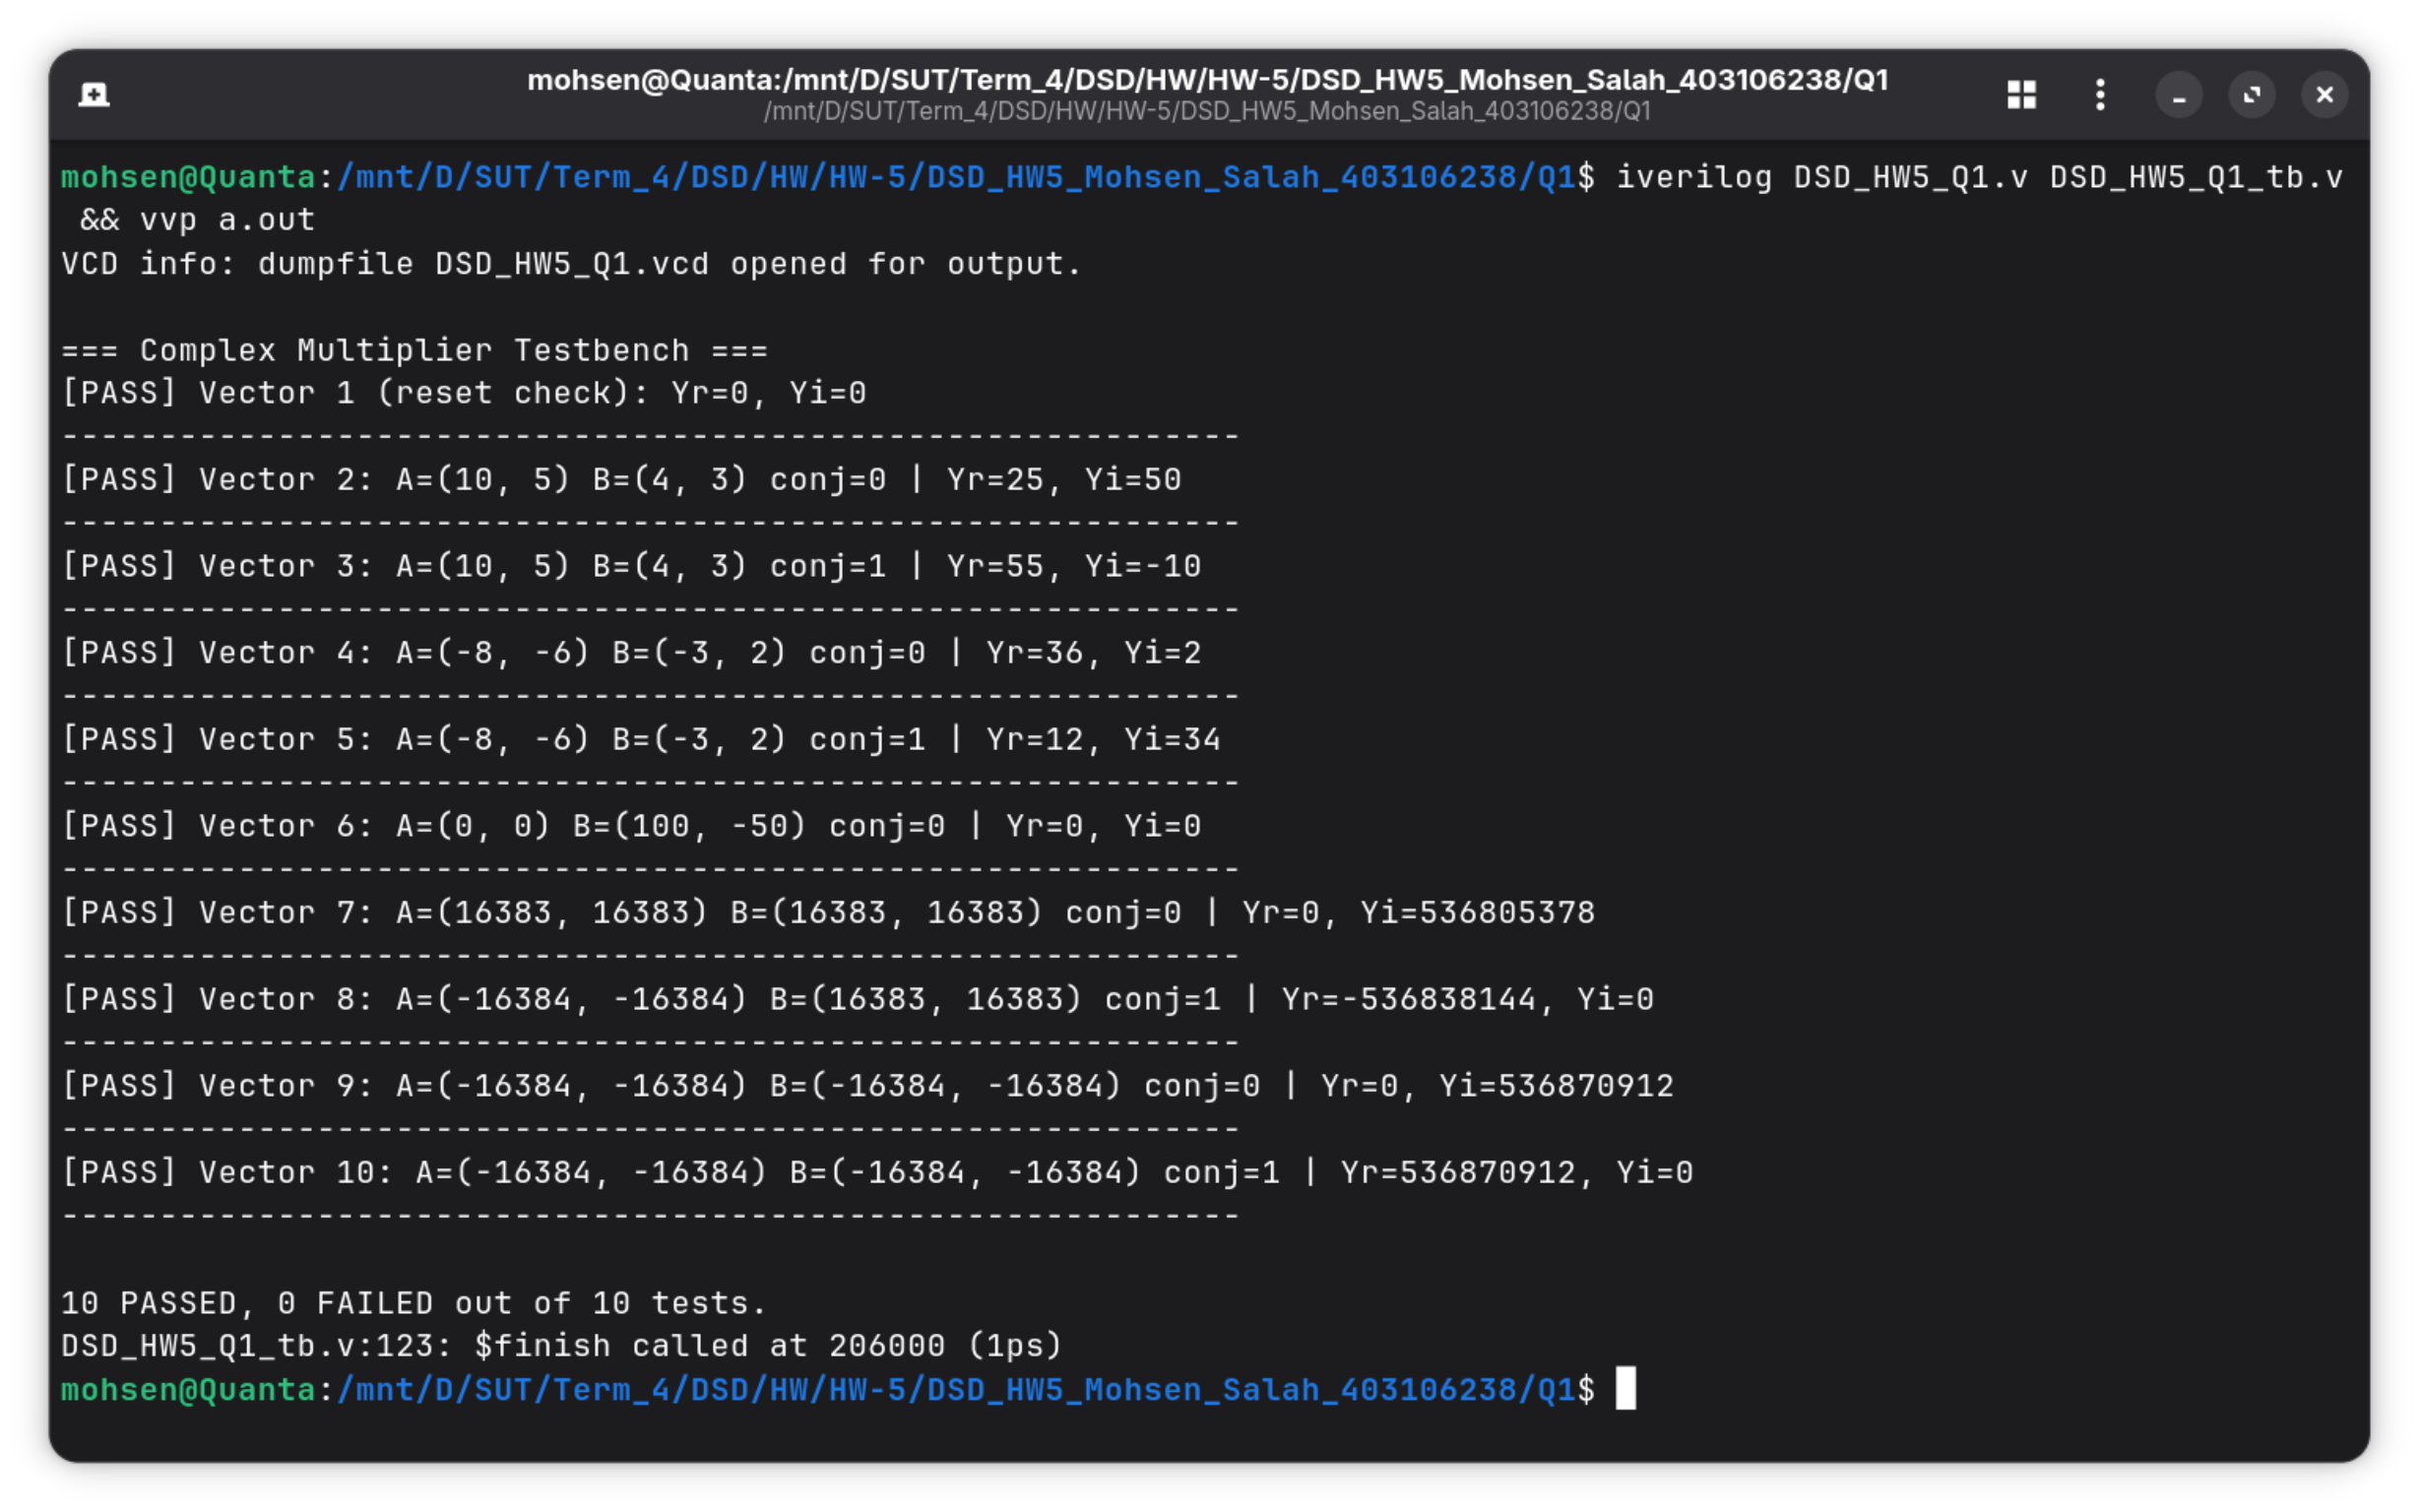
\includegraphics[width=1.0\textwidth]{assets/terminal.png}
    \caption{خروجی تست‌بنچ}
\end{figure}

همان طور که مشاهده می‌شود، تمام ۱۰ تست با موفقیت پاس شده‌اند.

\pagebreak

سیگنال‌ها را می‌توانیم در \lr{GTKWave} نیز بررسی کنیم:

\begin{figure}[H]
    \centering
    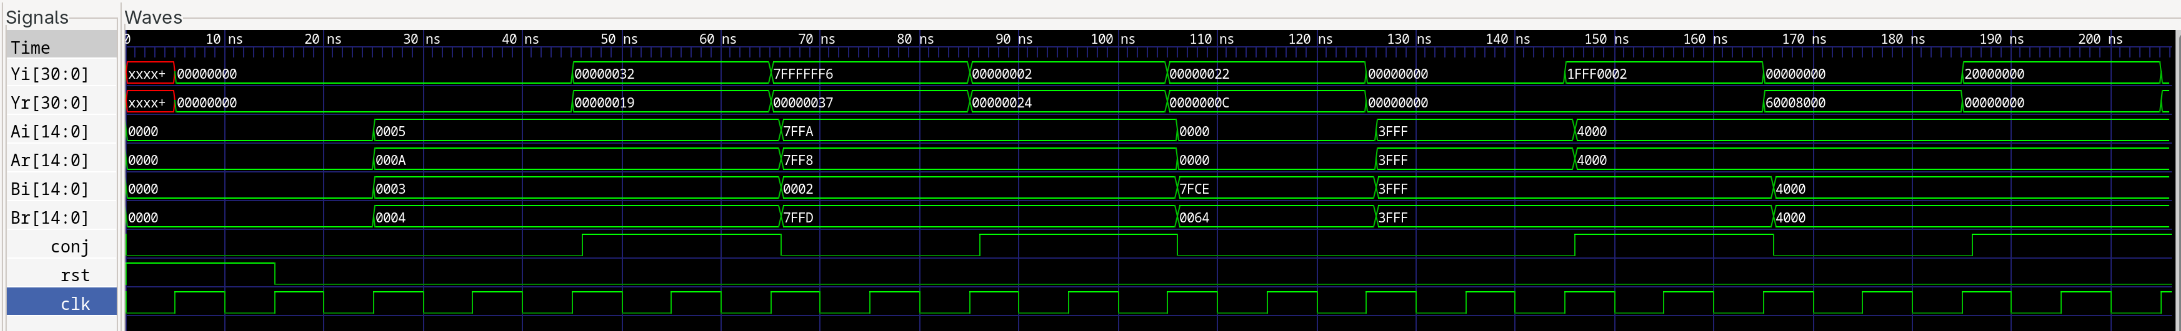
\includegraphics[width=1.0\textwidth]{assets/gtkwave.png}
    \caption{شکل موج سیگنال‌ها در \lr{GTKWave}}
\end{figure}

در موج‌نگار، تأخیر ۲ سیکل \lr{pipeline} به وضوح قابل مشاهده است: بعد از اعمال ورودی‌ها، خروجی دقیقاً دو لبه‌ی ساعت بعد آپدیت می‌شود.